\section{模型假设}

在不改变题给经验物性的前提下，作如下假设并明确其适用范围：

\begin{enumerate}[label=\arabic*)]
  \item 药材初始温度和干基含水率在内部均匀；材料轴对称，热物性和质扩散率在局部可视为各向同性标量。
  \item 主模型描述几何中截面的径向过程，端面取绝热、不透湿边界。题面未说明端面是否暴露，因此该条件作为模型假设；附录另用二维轴对称暴露端面对照检验其影响。
  \item 侧表面热交换满足牛顿冷却定律，水分交换满足线性Robin条件。问题二至四沿用题给$h$和$h_m$；主情景取$C_{\mathrm{eq}}=Y$，并通过宽范围比例系数$\beta$考察这一闭合对长期终点的影响。
  \item 将题给经验密度$\hat\rho(C)$仅用于构成有效体积热容$b(C)=\hat\rho(C)c_p(C)$。水分方程按干固体质量守恒建立，不把$\hat\rho/(1+C)$同时强制解释为严格干固体密度。
  \item 问题四仅发生径向仿射收缩，长度保持$25$ cm，材料速度与网格速度一致；半径$R(t)$由附件观测指定，而非由含水率反演。
  \item 忽略辐射、蒸发潜热、水分携带焓、形变功和化学反应。因而热方程是题设参数下的有效显热模型，其守恒残差不代表完整多相能量守恒。
\end{enumerate}

图\ref{fig:model-geometry}给出主模型的几何、边界与问题四坐标映射。固定域以薄环$V_i=\pi(r_{i+1/2}^2-r_{i-1/2}^2)L$为控制体，用两侧面通量之差闭合局部守恒；收缩域采用$\xi=r/R(t)\in[0,1]$，将移动物理边界映射为固定材料边界。本文的“全域”特指所建一维径向域，端面影响另作二维情景审查。

\begin{figure}[H]
  \centering
  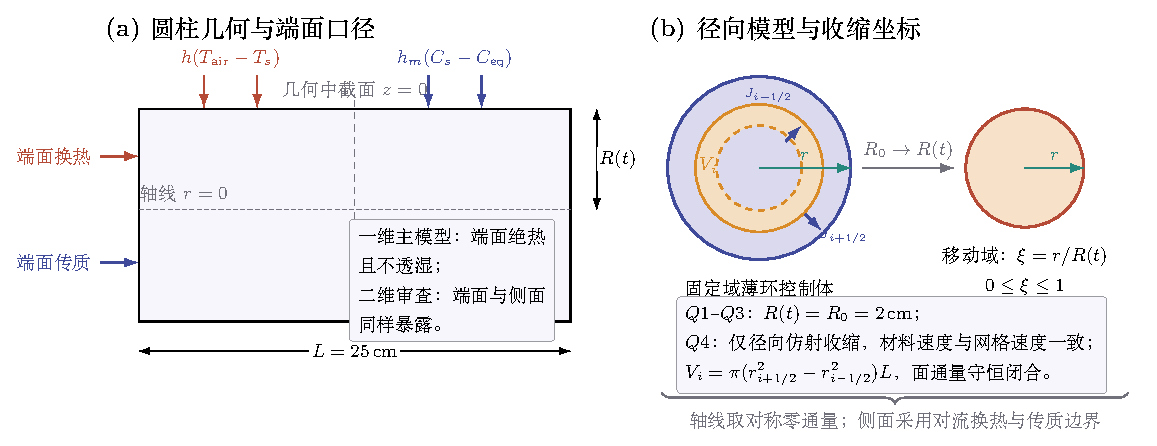
\includegraphics[width=0.92\textwidth]{figures/fig00b_model_geometry.pdf}
  \caption{几何边界与收缩坐标}
  \label{fig:model-geometry}
\end{figure}

\section{符号说明}

本文主要符号见表\ref{tab:symbols}。摄氏温度用于场值输出，只有经验指数中的温度使用绝对温度$T_K=T+273.15$。

\begin{table}[htbp]
  \caption{主要符号}
  \label{tab:symbols}
  \centering
  \begin{tabularx}{0.96\textwidth}{cXc}
    \toprule
    符号 & 含义 & 单位 \\
    \midrule
    $t$ & 自烘干开始的物理时间 & s \\
    $r,\ R(t),\ L$ & 径向坐标、当前半径、圆柱长度 & m \\
    $\xi$ & 材料参考坐标$r/R(t)$ & 1 \\
    $T,\ T_K$ & 摄氏温度与绝对温度 & $^\circ$C，K \\
    $C$ & 药材干基含水率 & kg/kg \\
    $Y,\ C_{\mathrm{eq}}$ & 环境水分量、药材侧等效边界含水率 & kg/kg \\
    $\hat\rho,\ c_p,\ b$ & 经验密度、比热容、有效体积热容 & kg/m$^3$，J/(kg$\cdot$K)，J/(m$^3\cdot$K) \\
    $k,\ \alpha$ & 导热系数、热扩散率$k/b$ & W/(m$\cdot$K)，m$^2$/s \\
    $D$ & 有效水分扩散率 & m$^2$/s \\
    $h,\ h_m$ & 对流换热系数、表面传质系数 & W/(m$^2\cdot$K)，m/s \\
    $\beta,\ S_p$ & 平衡边界比例系数、无量纲局部灵敏度系数 & 1 \\
    $s$ & 单位当前体积内的干固体质量 & kg/m$^3$ \\
    $v,\ w$ & 材料速度与移动网格速度 & m/s \\
    $\bar C,\ C_{\max}$ & 干质量加权平均与全域最大含水率 & kg/kg \\
    $t_*$ & $C_{\max}=0.15$的临界时刻 & s或h \\
    \bottomrule
  \end{tabularx}
\end{table}
